%%%%%%%%%%%%%%%%%%%%%%%%%%%%%%%%%%%%%%%%%%%%%%%%%%%%%%%%%%%%%%%%%%%
\section{Electron-positron plasma in BBN: damped-dynamic screening}\label{chap:bbn}

In this Chapter, we discuss the application of the non-relativistic limit of the polarization tensor in Chapter \ref{chap:PlasmaSF} to the electron-positron plasma which existed during Big Bang nucleosynthesis (BBN) as found in \cite{Grayson:2023flr} and reproduced in Appendix \ref{appendixC}. The BBN Epoch occurred within the first 20 min after the Big Bang when the Universe was hot and dense enough for nuclear reactions to produce light elements up to lithium \cite{Pitrou:2018cgg}. BBN reactions typically take place within the temperature interval $86\, \mathrm{keV}>\mathrm{T_{BBN}}>50\, \mathrm{keV}$~\cite{Pitrou:2018cgg}. We refer to these elements produced in BBN as primordial light elements to distinguish them from those made later in the Universe's history. Primordial light element abundances are the most accessible probes of the early Universe before recombination. Though the current BBN model successfully predicts D, $^3$ He, $^4$ He abundances, well-documented discrepancies, such as $^7$Li, remain. Efforts to resolve the theoretical BBN model with present-day observations are discussed in detail in \cite{Pitrou:2021vqr,Bertulani:2022qly}.

Huge electron-positron $e^-e^+$- number densities existed in the early Universe during Big Bang nucleosynthesis (BBN)~\cite{ Wang:2010px, Hwang:2021kno, Rafelski:2023emw} are $10^2$ times larger than those present in the sun \cite{bahcall2001solar} and $10^4$ times normal atomic densities \cite{Grayson:2023flr}. Charge screening is an essential collective plasma effect that modifies the internuclear potential $\phi(r)$ changing thermonuclear reaction rates during BBN. An electron cloud around an ion's charge effectively diminishes the influence of nuclear charges beyond their immediate vicinity, lowering the Coulomb barrier. In the context of nuclear reactions, a reduced Coulomb barrier leads to a higher likelihood of penetration, boosting thermonuclear reaction rates. Consequently, this process influences the abundance of light elements in the early universe by modifying their formation rates. Since the BBN temperature range is much less than the electron mass, we will use the non-relativistic limit of the polarization tensor derived in Chapter \ref{chap:PlasmaSF}. The screened potential relevant for thermonuclear reactions will be given by the longitudinal polarization function \req{eq:phi}.

The influence of screening on nuclear reactions is a well-established field of study. The concept of plasma screening effects on nuclear reactions was initially introduced in~\cite{Salpeter:1954nc}, who suggested determining the increase in nuclear reaction rates through the use of the static Debye-Hückel potential~\cite{Debye:1923,Salpeter:1969apj,Famiano:2016hhs}. Subsequent research expanded this framework to account for the thermal velocity of nuclei traversing the plasma~\cite{Hwang:2021kno,Carraro:1988apj, Gruzinov:1997as,Opher:1999jh,Yao:2016cjs}, introducing the concept of `dynamic' screening. In our current study, we address the high density of the $e^-e^+\gamma$ plasma by including collisional damping using the current conserving collision term developed in \cite{Formanek:2021blc} shown in \req{eq:collision}. The dense aspect of the BBN plasma has only recently been acknowledged by incorporating collision effects into numerical models \cite{Sasankan:2019oee,Kedia:2020xdc}. We will refer to this model of screening as 'damped-dynamic' screening. In \cite{Grayson:2023flr}, we find an analytic formula for the induced screening potential, which allows for estimating the enhancement of thermonuclear reaction rates.
 
% To improve the understanding of the internuclear screened Coulomb potential $\phi$ governing BBN reaction rates, this work expands the prior studies~\cite{Hwang:2021kno, Carraro:1988apj,Opher:1999jh, Yao:2016cjs} carried out in the linear response approximation applicable in the regime where the modification of the Coulomb potential is a small effect. We extend the 'dynamic screening' effort (and in particular that of Hwang et al~\cite{Hwang:2021kno} which introduced dynamic screening during BBN) to study `damped-dynamic' screening as follows:
% \begin{enumerate}
% \item 
% We detail the scattering damping effect of plasma components in the temperature range beginning near $T\simeq m_ec^2=511$\,keV extending down to a temperature near $T_\mathrm{split}\simeq 20.3$\,keV where practically all $e^-e^+$-pairs disappeared.
% \item 
% We obtain analytical results for damped-dynamic screening applicable to the BBN epoch temperature range which demonstrates a connection between the BBN plasma and dusty plasma theory. 
% \item 
% We recognize and describe the limits of applicability of the linear response method to BBN by considering the full equilibrium distribution necessary in the presence of strong fields. We explore a one-dimensional toy model at distances a fraction of an \AA ngstrom in the quantum tunneling regime where the potential $\phi$ is large compared to the thermal collision energy $|\phi|/3T> 1$,  which predicts enhanced screening at small distances.
% \end{enumerate}

% Such effort to improve the BBN model through screening is well justified for the following reasons:
% \begin{enumerate}
% \item Currently, the most accessible path to observe the early Universe before recombination is through light element abundances. 
% \item
% Despite the great initial success of the BBN model regarding the prediction of the abundances of D, $^3$ He, $^4$ He, there remain well-documented discrepancies. Currently, substantial efforts are being directed toward reconciling the theoretical BBN model with present-day observations. For a more detailed discussion, see Refs.\,\cite{Pitrou:2021vqr,Bertulani:2022qly}.
% \item
% Enhanced production of light elements during the BBN era could help resolve two problems: a) Elements Beryllium and Boron cannot be produced in stellar burning processes while their high abundance suggests additional mechanisms of production beyond secondary processes after stellar explosions. b) Understanding the age of stars obtained using the abundance of light elements (metallicity) may be improved by adaptation of the BBN network to account for nuclear reactions in ultra-dense QED plasma.
% \item
% We note that screening effects are more pronounced for nuclei with greater charge $Z$ leading to stronger modification in predicted abundances, just where the most significant current disagreements exist ({\it e.g.\/} the abundance of $^7$Li). Inclusion of screening effects in our current models of the BBN reaction network could explain this discrepancy without the need to invoke more exotic modifications of the Coulomb internuclear potential. An example of such a modification would be the variation of $\alpha$, the fine-structure constant~\cite{Meissner:2023voo}.
% \item 
% Recent James Webb space telescope-Hubble space telescope (JWST-HST) observations implying early onset of galactic structure formation and/or presence of luminous objects as early as 300 million years after BBN~\cite{Haro:2023JWST,Sabti:2023xwo,Ilie:2023DM} could be seen as evidence supporting nuclear dust matter clustering in dense QED plasma.
% \end{enumerate}


% In the standard BBN model, thermonuclear reaction rates are evaluated using nuclear reactions specific to the vacuum state. In a high-precision BBN model, the effect of $e^-e^+$-pair-plasma screening of nuclear charges must be allowed. We describe in Section~\ref{sec:density} the presence of up to several millions of electron-positron ($e^-e^+$) pairs per every charged nucleon. This situation prompts an effort to reconsider BBN in an ultra dense plasma environment allowing for a dense $e^-e^+\gamma$ plasma medium.

% We account for collisions between plasma components using the current-conserving Bhatnagar, Gross, and Krook (BGK) collision term~\cite{Bhatnagar:1954zz}, which allows us to study damping in the dynamic plasma. For an in-depth discussion presented in contemporary covariant notation and preserving current conservation, see Formanek et al.~\cite{Formanek:2021blc}. Our approach is different from Monte-Carlo simulation of two particle collisions~\cite{Sasankan:2019oee,Kedia:2020xdc} as in our case particles participating in scattering also experience simplified static screening which in terms of collision description would require more than two particle collisions. In addition, the simplified BGK collision term we employ allows us to obtain an analytic `damped-dynamic' internuclear potential relevant to the BBN reaction network in the linear response approximation. 

% Several well known processes, including M\o ller, Bhabha, and inverse Compton scattering, characterize the damping in plasma. These textbook results will be adapted to the plasma environment: When studied in vacuum, electrons and positrons interact with each other by exchanging a massless photon. However, when a photon propagates through a plasma of electrons and positrons, its properties are modified by interactions with the medium. When evaluating Moller and Bhabha scattering, we include the temperature-dependent mass of the photon obtained in plasma theory without damping. We find that the total relaxation rate during BBN is much larger than the screening mass, which is the inverse of the Debye screening length $m_D = 1/\lambda_D$. This suggests that electromagnetic perturbations of the plasma will be overdamped.

% Since, as noted above, the computed damping strength is the dominant scale, it is also the main parameter determining the photon mass. However, introducing the damping strength in the photon mass would make the calculation of the damping strength self-referential. The complexity of such a self-consistent evaluation of damping is beyond the scope of this work. This underscores the need to develop a self-consistent approach where both damping and photon properties in plasma are determined in a mutually consistent manner.

% The QED $e^+e^-\gamma$-plasma present during BBN is perturbed by a variety of comparatively very heavy charged protons $p$ and even heavier isotopes and light elements. In calculating the electromagnetic potential $\phi$, we naturally view BBN active participants as heavier, higher charged impurities {\it i.e.\/} \lq\lq charged dust\rq\rq in the QED-plasma. Since theories of such a system have been developed by others working on charged dust grains in planetary and space plasma~\cite{Montgomery:1970jpp, Stenflo:1973, Shukla:2002ppcf, Lampe:2000pop} we can validate our results and adapt previously developed theoretical tools necessary for describing heavy charged impurities within a plasma of lighter particles.

% We provide the first step in merging these two fields by including damping to analyze the electromagnetic potential during BBN, similar to work done by Stenflo in 1973 for dusty plasma~\cite{Stenflo:1973}. We advance this work by applying it to the BBN epoch, allowing for the finite size of the "dust grains," and by finding the short-distance behavior of the potential in the weak field limit. Using a general model of simplified collisional damping in linear response, we calculate the screened electromagnetic potential of light nuclei undergoing thermal motion subject to damping relying on previous work ~\cite{Formanek:2021blc,Grayson:2022asf}.

% Our manuscript is organized as follows: In Section~\ref{sec:density} we derive the electron-positron density and chemical potential to show that during the normal BBN temperature range $86\,\mathrm{keV}>\mathrm{T_{BBN}}>50\,\mathrm{keV}$~\cite{Pitrou:2018cgg} the Universe was filled with a dense electron-positron pair-plasma dotted with dispersed baryonic matter dust. 
% In Section~\ref{sec:relax}, we calculate the relaxation rate $\kappa= 1/\tau$, where $\tau$ is the mean time between collisions in the plasma. This is done by finding the average of the most relevant reaction rates for $2\leftrightarrow 2$ scattering: M{\o}ller, Bhabha, and inverse Compton scattering. 

% We proceed in Section~\ref{sec:kinetic_theory} to solve the Vlasov-Boltzmann Equation (VBE) in the weak field limit with damping. Our approach considers small plasma perturbations in linear response to find the polarization tensor present during the BBN era. In Section~\ref{sec:potential}, we find an analytic expression for the damped-dynamic potential applicable to BBN and study the limitation of the linear response method. We show that additional strong field phenomena beyond linear response alter the behavior of the screened potential $\phi$. We discuss our results and describe their interdisciplinary importance in Section~\ref{sec:Discussion}. 
 
%%%%%%%%%%%%%%%%%%%%%%%%%%%%%%%%%%%%%%%%%%%%%%%%%%%%%%%%%%%%%%%%%%%




\subsection{Early Universe plasma: non-relativistic polarization tensor}\label{sec:kinetic_theory}
The properties of the BBN plasma are described by the relativistic Vlasov-Boltzmann transport equations \req{eq:VBEf}. Since photons do not couple directly to the electromagnetic field, they do not contribute to the polarization tensor at first order in $\delta f$ as indicated in Eq.\,(\ref{eq:VBEg}). We neglect photon influence on the electron-positron distribution through the scattering term since the rate of inverse Compton scattering $R_{e^{\pm}\gamma }$ shown in green in \reff{RelaxationRate_fig} is much smaller, in the BBN temperature range, than the total rate $\kappa$ shown as a black line. Each fermion Boltzmann equation \req{eq:VBEf} can be solved independently. Since the equations for electrons and positrons are equivalent, except for the charge sign, only one needs to be solved to understand the dynamics.

We do not consider the influence of light nuclei on the polarization tensor since their density during the BBN epoch is much smaller than that of electrons and positrons \reff{BBN_Electron}. One can see in \reff{MeanFreePath_fig} that the separation of baryons $n_B^{-1/3}$ in black is much larger than the size of the polarizing Debye sphere, so baryons do not participate significantly in screening.

We take the equilibrium one particle distribution function $\eq{f_\pm}$ of electrons and positrons to be the relativistic Fermi-distribution
\begin{equation}\label{eq:equildist}
\eq{f}_\pm(p) = \frac{1}{\exp{\left(\frac{\sqrt{\boldsymbol{p}^2 + m^2}}{T}\right)}
+1}\,,
\end{equation}
with chemical potential $\mu = 0 $. The electron and positron mass will be indicated by $m$ unless otherwise stated. At temperatures interesting for nucleosynthesis $T = 50-86$\,keV, we expect the plasma temperature to be much less than the mass of the plasma constituents. Only the non-relativistic form of Eq.\,(\ref{eq:equildist}) will be relevant at these temperature scales
\begin{equation}
\eq{f}_\pm(p) \approx \exp\left(- \frac{m}{T}\left(1+\frac{|\pmb{p}|^2}{2m^2}\right)\right)\,.
\end{equation}
Keeping terms up to quadratic order in $|\boldsymbol{p}|/m$ we solve the Vlasov-Boltzmann equation Eq.\,(\ref{eq:VBEf}) for the induced current and identify the polarization tensor. This is done in detail in our previous work in~\cite{Formanek:2021blc}.

% First, we expand Eq.\,(\ref{eq:VBEf})
% around small perturbations from equilibrium
% \begin{equation}\label{eq:perturbation0}
% f_\pm(x,p) = {\eq{f}_\pm}(p) + \delta f_\pm(x,p)\,,
% \end{equation}
% and solve \req{eq:VBEf} for $\delta f_\pm(x,p)$ in Fourier space. The induced current in Fourier space is given by
% \begin{equation}\label{eq:perturbation1}
% \tilde{j}_{\mathrm{ind}}^\mu(k) = 2\int \frac{d^4 p}{(2 \pi)^4}p^\mu 4\pi \delta_+(p^2-m^2) 
% \sum_{i = \, +, \, -} q_i \tilde{f}_{i}(k,p)\,,
% \end{equation}
% with the factor of two accounting for spin.
% After inserting \req{eq:perturbation0}, and specifying $q_\pm = \pm e$ the induced current is a function of the perturbation
% \begin{multline}\label{eq:perturbation2}
% \tilde{j}_{\mathrm{ind}}^\mu(k) = 2\int \frac{d^3 p}{(2 \pi)^3 p^0}p^\mu \Big( e \left[\eq{\tilde{f}}_+(k,p)-\eq{\tilde{f}}_-(k,p)\right]\\
% + e\left[\delta\tilde{f}_+(k,p)-\delta\tilde{f}_-(k,p)\right]
% \Big)
% \\
% =4 e\int \frac{d^3 p}{(2 \pi)^3 p^0}p^\mu \delta\tilde{f}(k,p)
% \,,
% \end{multline}
% because the equilibrium currents cancel in the weak field limit and the perturbations add since they differ by the charge $\delta f_\pm=\pm e \delta f' $. This term is studied for finite chemical potential in~\cite{Wang:2010px}. We focus on the second term related to the polarization response of the plasma.

% The polarization tensor can be obtained from \req{eq:perturbation2} by computing the 4-momentum integrals over $p$ in the rest frame of the plasma. Once integrated, the 4-potential $\widetilde{A}^{\nu}(k)$, coming from the electromagnetic field strength tensor $F^{\mu \nu}$ in \req{eq:VBEf}, factors out since it only depends on the 4-wavevector $k$ and \req{eq:perturbation2} attains the form of \req{eq:linresp}. For details, see Ref.~\cite{Formanek:2021blc}.

In the infinite homogeneous plasma filling the early Universe, the polarization tensor only has two independent components: the longitudinal polarization function $\Pi_{\parallel}$ parallel to field wave-vector $\boldsymbol{k}$ in the rest frame of the plasma and the transverse polarization function $\Pi_{\perp}$ perpendicular to $\boldsymbol{k}$~\cite{melrose2008quantum}. In the non-relativistic limit, these functions are~\cite{Formanek:2021blc}
\begin{align}\label{eq:polfuncs}
	\Pi_\parallel(\omega,\boldsymbol{k}) &= -\omega_p^2\frac{\omega^2}{(\omega+ i \kappa)^2} \frac{1}{1-\frac{i\kappa}{\omega+ i \kappa}\left(1+\frac{ T |\boldsymbol{k}|^2}{m (\omega+ i \kappa)^2} \right)}\,,\\
	\Pi_{\perp}(\omega) &= -\omega_p^2 \frac{\omega}{\omega+ i \kappa}\,.
\end{align}
In these expressions, the plasma frequency $\omega_p$ (defined as $m_L$ in~\cite{Formanek:2021blc}) is related to the Debye screening mass in the non-relativistic limit as
\begin{equation}\label{eq:plasmafreq}
 \omega_p^2 = m_D^2\frac{T}{m}\,.
\end{equation}

\begin{figure}[ht]
\begin{center}
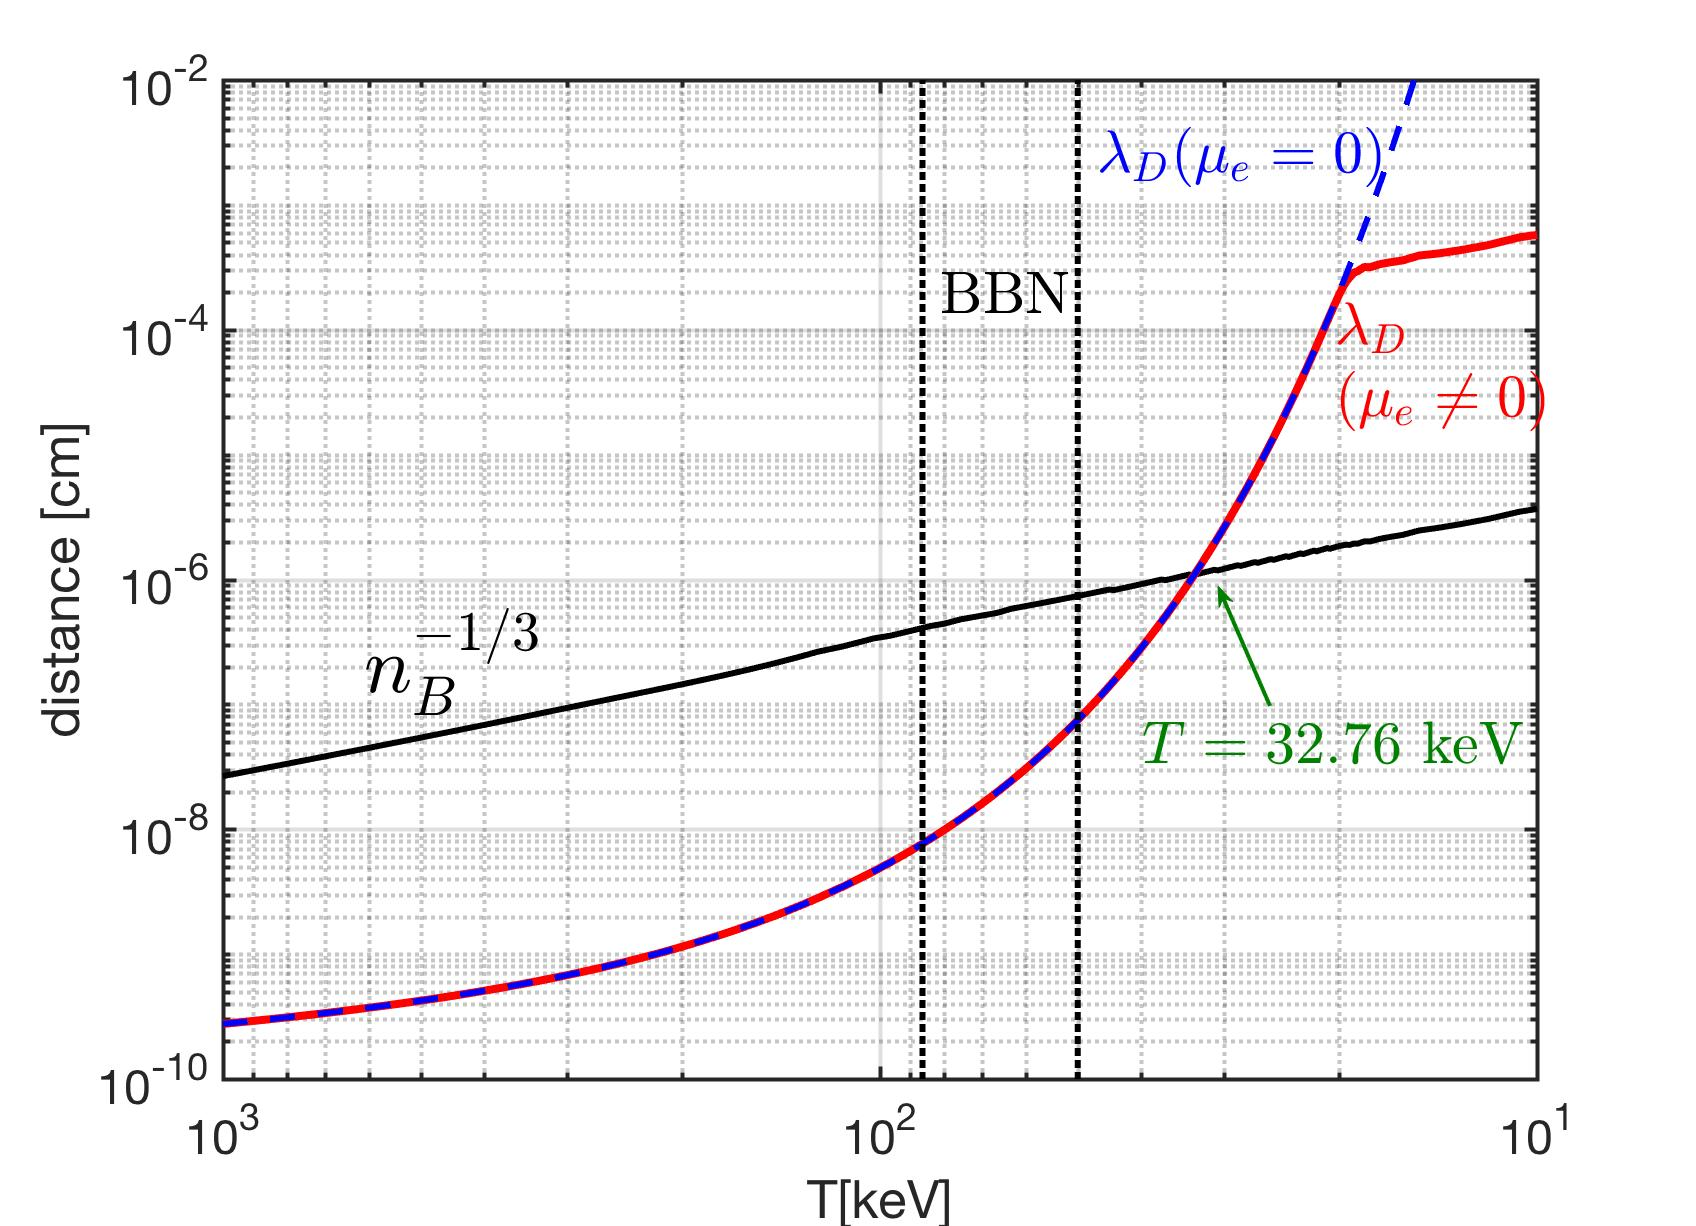
\includegraphics[width=0.95\linewidth]{plots/chap03BBN/Distance_Plasma002.jpg}
\caption{\textit{From \cite{Grayson:2023flr}; figure by C. T. Yang.} The average distance between baryons $n_B^{-1/3}$ and the Debye length $\lambda_D$ ($\mu_e \neq 0$) as a function of temperature (red solid line). During the BBN epoch (vertical dotted lines) $n_B^{-1/3}>\lambda_D$. For temperature below $T<32.76$ keV we have $n_B^{-1/3}<\lambda_D$. For comparison, the Debye length for zero chemical potential $\mu_e=0$ is also plotted as a blue dashed line.}
\label{MeanFreePath_fig}
\end{center}
\end{figure}
%~~~~~~~~~~~~~~~~~~~~~~~~~~~~~~~~~~~~~~~~~~~~~

The transverse response $\Pi_{\perp}$ relates to the dispersion of photons in the plasma. Here we need only consider $\Pi_\parallel$ since the vector potential $\boldsymbol{A}(t,\boldsymbol{x})$ of the traveling ion will be small in the non-relativistic limit. This work does not consider the effect of a primordial magnetic field discussed in~\cite{Steinmetz:2023abc}. We note that Debye mass $m_D$ is related to the usual Debye screening length of the field in the plasma as
\begin{equation}\label{eq:mL}
	1/\lambda_D^{2} = m_D^2= 4 \pi \alpha \left(\frac{2mT}{\pi}\right)^{3/2}\frac{e^{-m/T}}{2T}\,.
\end{equation}
This formula describes the characteristic length scale of screening in the plasma.

\subsection{Longitudinal dispersion relation}
As discussed in Chapter \ref{chap:PlasmaSF} the poles in the propagator or roots of the dispersion equation represent the plasma's propagating modes, often called `quasi-particles' or 'plasmons.' In the non-relativistic limit, one can solve the longitudinal part of the dispersion equation \req{eq:disp}, which is relevant for finding charge oscillation modes in the plasma
\begin{equation}
    1+ \frac{\Pi_\parallel( k)}{(p\cdot u)^2}= 1+ \frac{\Pi_\parallel(\omega, \boldsymbol{k})}{\omega^2}=\varepsilon_\parallel(\omega,\boldsymbol{k}) =0 \,,
\end{equation}
evaluated in the rest frame. Then we insert \req{eq:polfuncs} to find
\begin{equation}
   1- \frac{\omega_p^2}{(\omega+ i \kappa)^2} \frac{1}{1-\frac{i\kappa}{\omega+ i \kappa}\left(1+\frac{T |\boldsymbol{k}|^2}{m(\omega+ i \kappa)^2} \right)}=0 \,.
\end{equation}
We can simplify the above expression since this is only a function of $\omega' =\omega+i\kappa$
\begin{equation}
   1- \frac{\omega_p^2}{\omega'^2-i\kappa\omega'+\frac{i\kappa T |\boldsymbol{k}|^2}{m \omega'} }=0 \,.
\end{equation}
Then we get a cubic equation for $\omega'(|\boldsymbol{k}|)$
\begin{equation}\label{eq:dispfact}
   \frac{1}{\omega'^3-i\kappa\omega'^2+\frac{i\kappa T |\boldsymbol{k}|^2}{m} }
    \left(\omega'^3-i\kappa\omega'^2 - \omega_p^2\omega'+\frac{i\kappa T |\boldsymbol{k}|^2}{m} \right)=0 \,.
\end{equation}
Cardano's formula gives the solutions to this cubic equation
\begin{equation}\label{eq:cardano}
\omega_n(\boldsymbol{k}) = \frac{1}{3}\left(i\kappa-\xi^n C-\frac{\Delta_0}{\xi^n C}\right), \qquad n \in \{0,1,2\} \,,
\end{equation}
with the quantities:
\begin{align}\label{eq:delta}
  \xi &=\frac{i\sqrt{3}-1}{2}\,,\\
    C &= \sqrt[3]{\frac{\Delta_1 \pm \sqrt{\Delta_1^2 - 4 \Delta_0^3}}2}\,,\\
    \Delta_0 &= -\kappa^2 + 3 \omega_p^2\,,\\
\Delta_1 &= 2i\kappa^3 - 9 i\kappa \omega_p^2 + 27\frac{i\kappa T |\boldsymbol{k}|^2}{m}.
\end{align}
Since the longitudinal dispersion relation is analytically solvable the full non-relativistic potential can be found in position space using contour integration. The residue of each pole will lead to the strength of that mode, and the location of the pole will lead to space and time dependence, which in simple cases is exponential. In practice, factoring out these roots in the Fourier transform of the potential leads to five poles, which do not seem to lead to simple expressions in position space. We found using the approximate expression derived in \req{sec:potential} was more practical. Deriving the full expression is the subject of future work.

%\begin{figure}[H]
%    \centering
%    \includegraphics[width=0.95\linewidth]{plasmafreq.png}
%    \caption{Plot of the plasma frequencies $\omega_\pm$ in the complex plane as a function of $\kappa$. At $\kappa=2\omega_p$ both solutions become imaginary, one becoming more quickly damped and the other more slowly damped.}
%    \label{fig:plasma-freq}
%\end{figure}



\section{Effective internuclear potential}\label{sec:potential}
We calculate the potential of light nuclei in the early Universe electron-positron plasma by Fourier transforming the screened scalar potential $\phi$ of a single traveling nuclei \req{eq:phi}
\begin{equation}\label{eq:potent}
 \phi(t,\boldsymbol{x}) = \int \frac{d^4k}{(2\pi)^4} e^{-i\omega t+ i\boldsymbol{k}\cdot\boldsymbol{x}} \frac{\widetilde{\rho}_\text{ext}(\omega,\boldsymbol{k})}{\varepsilon_\parallel(\omega,\boldsymbol{k})(\boldsymbol{k}^2-\omega^2) }\,,
\end{equation}
where $\widetilde{\rho}_{\text{ext}}(\omega,\boldsymbol{k})$ is the Fourier-transformed charge distribution of nuclei traveling at a constant velocity, and $\varepsilon_\parallel(\omega,\boldsymbol{k})$ is the longitudinal relative permittivity. The relative permittivity can be written in terms of the polarization tensor as
\begin{equation}\label{eq:epsilon}
 \varepsilon_\parallel(\omega,\boldsymbol{k})= \left(\frac{\Pi_{\parallel}(\omega,\boldsymbol{k})}{ \omega^2}+1\right)\,.
\end{equation}

In the linear response framework \req{eq:ohm}, the electromagnetic field still obeys the principle of superposition so the potential between two nuclei can be inferred simply from the potential of a single nucleus. 

We can perform the $\omega$ integration in \req{eq:potent} using the delta function in the definition of the external charge distribution, whose effect is to set $\omega = \boldsymbol{\beta_{\text{N}}}\cdot \boldsymbol{k}$ where $\boldsymbol{\beta}_N = \boldsymbol{v}_N/c$ is the nuclei velocity. Then we have
\begin{equation}\label{eq:potentk}
 \phi(t,\boldsymbol{x}) = Ze\int \frac{d^3\boldsymbol{k}}{(2\pi)^3} e^{ i\boldsymbol{k}\cdot(\boldsymbol{x}-\boldsymbol{\beta_{\text{N}}} t)} \frac{ e^{-\boldsymbol{k}^2\frac{R^2}{4}}}{\boldsymbol{k}^2\varepsilon_\parallel(-\boldsymbol{\beta_{\text{N}}} \cdot \boldsymbol{k},\boldsymbol{k}) }\,,
\end{equation}
where $R$ is the Gaussian radius parameter.
In non-relativistic approximation the Lorentz factor $\gamma \approx 1$ and we use the convention $\varepsilon_\parallel(-\boldsymbol{\beta_{\text{N}}} \cdot \boldsymbol{k},\boldsymbol{k})$ used in~\cite{Montgomery:1970jpp, Stenflo:1973,Shukla:2002ppcf,Shukla1996} which gives the correct causality for the potential. This ensures that, without damping, the wakefield occurs behind the moving nucleus.

%%%%%%%%%%%%%%%%%%%%%%%%%%%%%%%%%%%%%%%%%%%%%%%%%%%%%%%%%%%%%%%%%%%%%%%%%%%%%%%
\subsection{Damped-dynamic screening}\label{sec:DDS}
This section presents the effective nuclear potential for a light nucleus moving in the plasma at a constant velocity. This is done by Fourier transforming \req{eq:potentk}. The velocity of the nucleus is assumed to be the most probable velocity given by a Boltzmann distribution
\begin{equation}\label{eq:vel}
 \beta_{\text{N}} = \sqrt{\frac{2T}{m_N}}\,. 
\end{equation}
Since the poles of the \req{eq:potent} can be solved analytically, ideally, one would perform contour integration to get the position space field. Due to the intricacy of these poles $\omega_n(\boldsymbol{k})$, we find it insightful to look at the field in a series expansion around velocities of the light nuclei smaller than the thermal velocity of electrons and positrons and large damping.

% \begin{equation}
% \beta_{\text{N}}\frac{m_D}{\kappa} = \frac{v_{\text{N}}}{c}\frac{m_D}{\kappa} \ll 1\,.
% \end{equation}
\begin{equation}\label{eq:expansion}
% (\boldsymbol{k}\cdot\boldsymbol{\beta}_{\text{N}})^2 \ll \boldsymbol{k}^2 \frac{T}{m} \ll \kappa^2\, 
\frac{(\boldsymbol{k}\cdot\boldsymbol{\beta}_{\text{N}})^2}{\omega_p^2} \ll \frac{\boldsymbol{k}^2}{m_D^2} \ll \frac{\kappa^2}{\omega_p^2}\, .
\end{equation}


This expansion is useful during BBN since the temperature is much lower than the mass of light nuclei and the damping rate $\kappa$ is approximately twice the Debye mass $m_D$, as seen in Fig.~\ref{RelaxationRate_fig}. Applying this expansion to \req{eq:potentk} and evaluating this expression for a point charge $r \rightarrow 0$ we find
% % \begin{multline} \label{eq:potexp}
% % \phi(t,\boldsymbol{x}) = \phi_{\text{stat}}(t,\boldsymbol{x}) +\\ -Ze\int \frac{d^3\boldsymbol{k}}{(2\pi)^3} e^{ i\boldsymbol{k}\cdot(\boldsymbol{x}-\boldsymbol{\beta_{\text{N}}} t)}\frac{i \boldsymbol{k}\cdot \boldsymbol{\beta_{\text{N}}} m_D^2 (\frac{\boldsymbol{k}^2}{\kappa} - \frac{m}{T} \kappa)}{\boldsymbol{k}^2(\boldsymbol{k}^2+m_D^2)^2} e^{-\boldsymbol{k}^2\frac{R^2}{4}} \\ + O
% % \left(\beta_{\text{N}}\frac{m_D}{\kappa}^2\right)\,.
% % \end{multline}
% \begin{multline} \label{eq:potexp}
%  \phi(t,\boldsymbol{x}) = \phi_{\text{stat}}(t,\boldsymbol{x})\\ -Ze\int \frac{d^3\boldsymbol{k}}{(2\pi)^3} e^{ i\boldsymbol{k}\cdot(\boldsymbol{x}-\boldsymbol{\beta_{\text{N}}} t)}\frac{i \boldsymbol{k}\cdot \boldsymbol{\beta_{\text{N}}} m_D^4 (\frac{\boldsymbol{k}^2}{m_D^2} - \frac{\kappa^2}{\omega_p^2})}{\boldsymbol{k}^2(\boldsymbol{k}^2+m_D^2)^2\kappa} e^{-\boldsymbol{k}^2\frac{R^2}{4}} \,.
% \end{multline}
% First, we focus on the second term evaluating for a point charge $R\rightarrow 0$
\begin{equation}\label{eq:ddsint}
\phi(t,\boldsymbol{x}) =\phi_{\text{stat}}(t,\boldsymbol{x})-Ze\int \frac{d^3\boldsymbol{k}}{(2\pi)^3} e^{ i\boldsymbol{k}\cdot(\boldsymbol{x}-\boldsymbol{\beta_{\text{N}}} t)}\frac{i \boldsymbol{k}\cdot \boldsymbol{\beta_{\text{N}}} m_D^4 (\frac{\boldsymbol{k}^2}{m_D^2} - \frac{\kappa^2}{\omega_p^2})}{\boldsymbol{k}^2(\boldsymbol{k}^2+m_D^2)^2\kappa}\,.
\end{equation}
The second term is the damped-dynamic screening correction which we refer to as $\Delta \phi$ where
\begin{equation}\label{eq:pos_point}
\phi(t,\boldsymbol{x}) = \phi_{\text{stat}}(t,\boldsymbol{x}) +\Delta \phi(t,\boldsymbol{x}) \,,
\end{equation}
and $\phi_{\text{stat}}$ is the standard static screening potential. The details of the integration of \req{eq:ddsint} can be found in \cite{Grayson:2023flr} in Appendix \ref{appendixC}, the result is
% In order to perform this integration we first note that this expression can be re-written as the laboratory time derivative
% \begin{equation}
%  \Delta\phi(t,\boldsymbol{x}) = Ze\frac{d}{dt}\left[\int \frac{d^3\boldsymbol{k}}{(2\pi)^3} e^{ i|\boldsymbol{k}||\boldsymbol{x}-\boldsymbol{\beta_{\text{N}}} t| \cos(\theta)}\frac{ m_D^4 (\frac{\boldsymbol{k}^2}{m_D^2} - \frac{\kappa^2}{\omega_p^2})}{\boldsymbol{k}^2(\boldsymbol{k}^2+m_D^2)^2\kappa}\right] \,,
% \end{equation}
% where the dot products were replaced by their angular dependence.
% The angular integration can be evaluated in spherical coordinates, see \ref{sec:static} for details,
% \begin{equation}
%  \Delta\phi(t,\boldsymbol{x}) = 2 Ze\frac{d}{dt}\left[\int \frac{d\boldsymbol{k}}{(2\pi)^2} \frac{\sin(|\boldsymbol{k}||\boldsymbol{x}-\boldsymbol{\beta}_N t|)}{|\boldsymbol{k}||\boldsymbol{x}-\boldsymbol{\beta}_N t|}\,\frac{ m_D^4 (\frac{\boldsymbol{k}^2}{m_D^2} - \frac{\kappa^2}{\omega_p^2})}{\boldsymbol{k}^2(\boldsymbol{k}^2+m_D^2)^2\kappa}\right] \,,
% \end{equation}
% \begin{multline}
%  \Delta\phi(t,\boldsymbol{x}) = \frac{Ze }{4\pi }\frac{m_D^2}{\kappa}\frac{d}{dt}\Bigg[\left(\frac{1+\nu_\tau^2}{ 2m_D}+\frac{\nu_\tau^2}{m_D^2 |\boldsymbol{x}-\boldsymbol{\beta}_N t|}\right)e^{-m_D |\boldsymbol{x}-\boldsymbol{\beta}_N t|}\\ - \frac{\nu_\tau^2}{m_D^2 |\boldsymbol{x}-\boldsymbol{\beta}_N t|} \Bigg]\,,
% \end{multline}
% here we introduce the ratio of the damping rate to the rate of oscillations in the plasma $\nu_\tau = \kappa/\omega_p$. We can apply the time derivative; note that
% \begin{equation}\label{eq:der_cos}
%  \frac{d}{dt} |\boldsymbol{x}-\boldsymbol{\beta}_N t| = - \frac{\boldsymbol{\beta}_N \cdot (\boldsymbol{x}-\boldsymbol{\beta}_N t)}{|\boldsymbol{x}-\boldsymbol{\beta}_N t|}= -\beta_N \cos(\psi)\,,
% \end{equation}
% where $\psi$ is the angle between $\boldsymbol{x}-\boldsymbol{\beta}_N t$ and $\boldsymbol{\beta}_N$. After taking the derivative and using the above expression \req{eq:der_cos} one finds

\begin{figure}[h!]
 \centering
 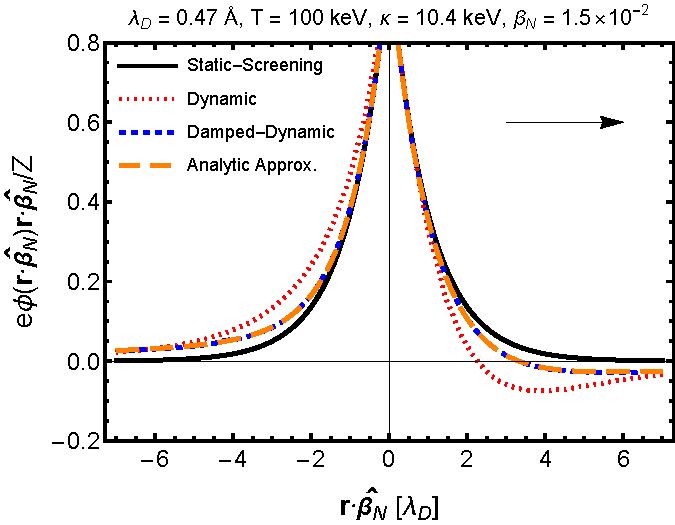
\includegraphics[width=.95\linewidth]{plots/chap03BBN/phidat_100_1_1_0_full.pdf}
 \caption{\textit{from \cite{Grayson:2023flr}}. Plot of the total screening potential scaled with charge Z and distance along the direction of motion. We show a comparison of the following screening models plotted along the direction of motion of a nucleus $\boldsymbol{r}\cdot\hat{\boldsymbol{\beta}_{\text{N}}}$: static screening (black), dynamic screening (red dotted) from \cite{Hwang:2021kno}, damped-dynamic screening (blue dashed), and the approximate analytic solution of \req{eq:pos_point} (orange dashed). A black arrow indicates the direction of motion of the nucleus $\hat{\boldsymbol{\beta}_{\text{N}}}$. }
 \label{fig:dynamiclinear}
\end{figure} 

\begin{multline}\label{eq:pos_point_DDS}
\Delta \phi(t,\boldsymbol{x}) = \frac{Ze \beta_N \cos (\psi) m_D^2}{4 \pi \varepsilon_0 \kappa} \Bigg[\left(\frac{\nu_\tau^2}{m_D^2 r(t)^2} + \frac{\nu_\tau^2}{m_D r(t)}+\frac{1 + \nu_\tau^2}{2}\right)e^{-m_D r(t)} \\ -\frac{\nu_\tau^2}{m_D^2 r(t)^2}\Bigg]\,,
\end{multline}
where $\psi$ is the angle between $\boldsymbol{x}-\boldsymbol{\beta}_N t$ and $\boldsymbol{\beta}_N$ and $r(t) = |\boldsymbol{x}-\boldsymbol{\beta}_N t|$.
We introduce the ratio of the damping rate to the rate of oscillations in the plasma $\nu_\tau = \kappa/\omega_p$.  This expression is valid for large damping and slow motion of the nucleus or if the velocity of the nuclei is small. A similar result valid at large distances, which only includes the last term, was previously derived in~\cite{Stenflo:1973} for dusty (complex) plasmas. For large distances and large $\nu_\tau$, the last term in the second line is dominant, indicating that the overall potential would be over-damped. In this regime, the potential is heavily screened in the forward direction and unscreened in the backward direction relative to the motion of the nucleus. As $\nu_\tau$ becomes small, the $1/2$ in the first portion of the third term, proportional to $m_D^2/\kappa$, dominates. This flips the sign of the damped-dynamic screening contribution causing a wake potential to form behind the nuclei. This shift indicates the change from damped to undamped screening where \req{eq:pos_point_DDS} is no longer valid. 

\begin{figure}[h!]
 \centering
 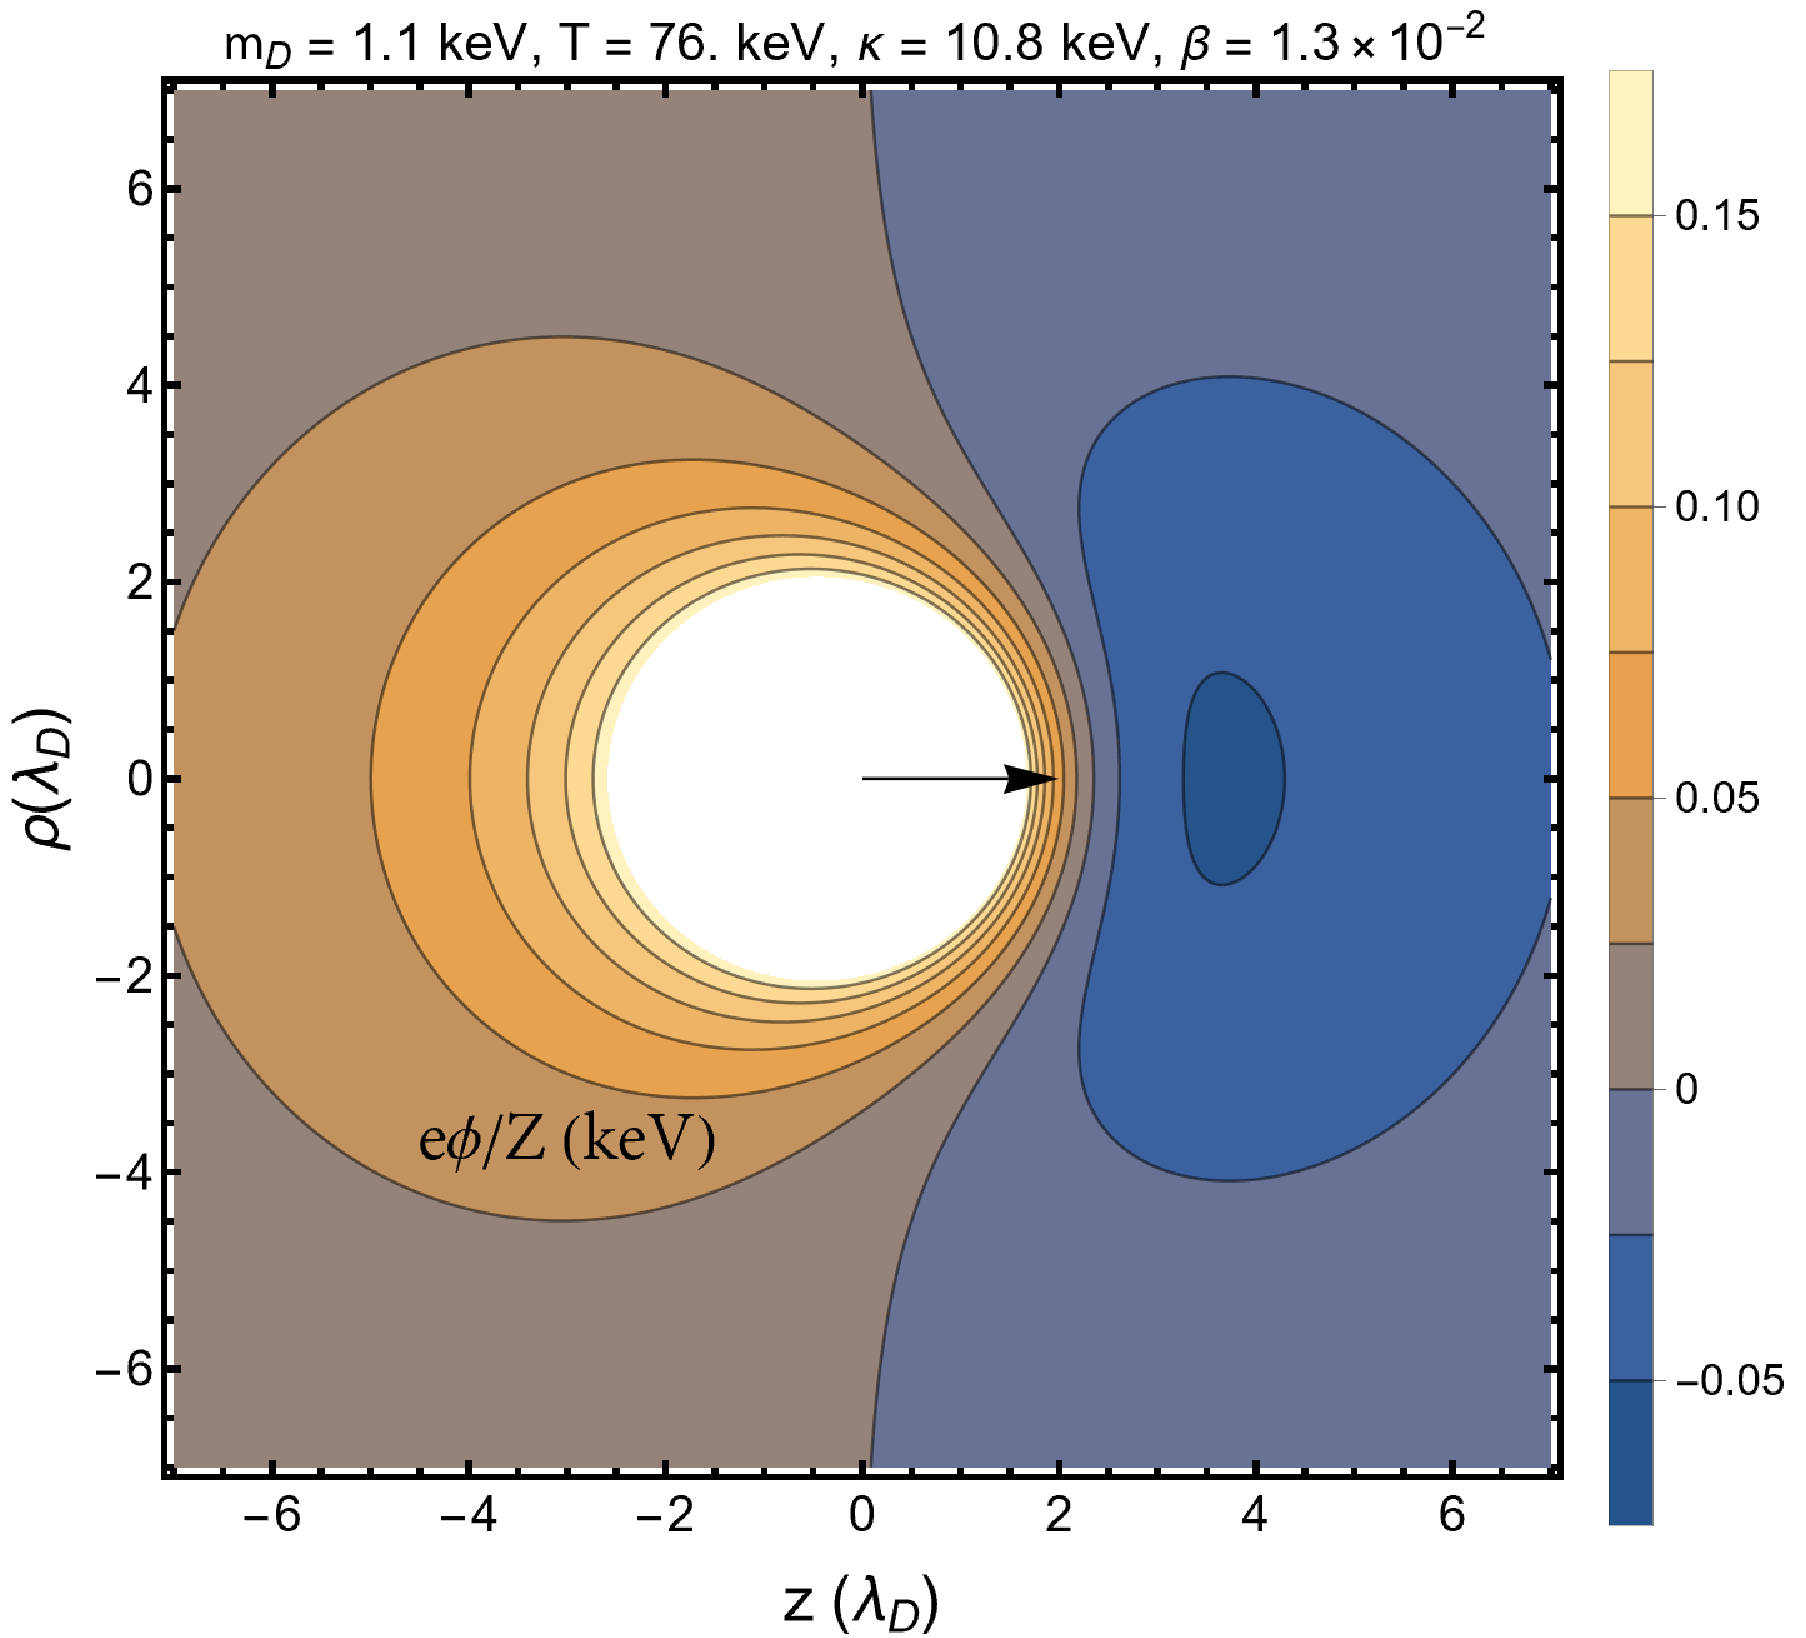
\includegraphics[width=.85\linewidth]{plots/chap03BBN/Pot_2DPlotFix.png}
 \caption{Two dimensional plot of the total potential \req{eq:pos_point} scaled with Z, at $T=74\,$keV. The potential is cylindrically symmetric about the direction of motion $\boldsymbol{\hat{z}}$, which is indicated by a black arrow. The direction transverse to the motion is $\rho$. The sign of the damped-dynamic correction \req{eq:pos_point_DDS} changes sign due to the cosine term.}
 \label{fig:numericalComp}
\end{figure} 

Figure \ref{fig:dynamiclinear} demonstrates that the damped-dynamic response in the analytic approximation \req{eq:pos_point_DDS} (shown as orange dashed line) is sufficient to approximate the full numerical solution (blue dashed line) found by numerical integration of \req{eq:potent}. The temperature $T = 100$\, keV, above our upper limit of BBN temperatures, is chosen to relate to the dynamic screening result found in~\cite{Hwang:2021kno}. Our analytic solution differs from the numerical result in Fig.~4 of \cite{Hwang:2021kno} by a factor of $\sqrt{2}$ and is horizontally flipped. This reflection is due to a difference in convention in the permittivity, as seen in \req{eq:potentk}. We can see that dynamic screening is slightly stronger at large distances than damped screening, as expected. Damped and undamped screening are very similar at short distances, which is relevant to thermonuclear reaction rates. 

Dynamic screening in both the damped and undamped cases predicts less screening behind and more in front of the moving nucleus than static screening. This is shown in the two-dimensional plot \reff{fig:numericalComp}, of the total potential in plasma at $T=76\,$keV This effect was previously observed for subsonic screening in electron-ion-dust plasmas ~\cite{Stenflo:1973, Shukla:2002ppcf, Lampe:2000pop}. As a result, a negative polarization charge builds up in front of the nucleus. The small negative potential in front alters the potential energy between light nuclei, possibly changing the equilibrium distribution of light elements in the early universe plasma. This effect is much larger in the undamped case and is known in some cases to lead to the formation of dust crystals~\cite{Shukla1996}. 

\section{Reaction rate enhancement}
We use the same argument as \cite{Salpeter:1954nc} to find the enhancement factor due to damped-dynamic screening. The enhancement of a nuclear reaction process by screening is related to the WKB probability of tunneling through the Coulomb barrier
\begin{equation} \label{eq:penprob}
    P(E) = \exp{\left( - \frac{2\sqrt{2 \mu_r}}{\hbar c}\int_{R}^{r_c}dr \sqrt{U(r)-E}\right)}\,,
\end{equation}
often referred to as the penetration factor. $U(r)$ is the potential energy of the two colliding nuclei, $\mu_r$ is their reduced mass, $E$ is the relative energy of the collision, $R$ is the radius of the nucleus, and $r_c$ is the classical turning point. In the weak screening limit, the screening charge density varies on the scale of $\lambda_D$, which is here on the order of \AA ngstrom. The distance scales relevant for tunneling are between $R$ and $r_c$, which is on the order of $10\,$fm. This allows us to approximate the contribution to the potential energy from screening, $H(r)$ defined as
\begin{equation}
    H(r) \equiv U(r) - U_\text{vac}(r)\,,
\end{equation}
as constant over the integral in \req{eq:penprob} taking the value of \req{eq:pos_point_DDS} at the origin,
\begin{equation}
     H(0) = Z_1\phi_2(0) = Z_1 Z_2 \alpha \left(m_D - \frac{\beta_N m_D^2}{2 \kappa}\right)\,.
\end{equation}
Then the screening effect reduces to a constant shift in the relative energy $E \rightarrow E+H(0)$. In this approximation, the enhancement to reaction rates can be represented by a single factor \cite{Salpeter:1954nc, PhysRevC.89.015802}
\begin{equation}\label{eq:DDSenhance}
   \mathcal{F} = \exp\left[\frac{H(0)}{T} \right]=\exp\left[\frac{Z_1 Z_2 \alpha}{T} \left(m_D - \frac{\beta_N m_D^2}{2 \kappa}\right)\right]\,.
\end{equation}
The first term is the normal weak field screening result, and the second is the contribution of damped-dynamic screening. Due to the large damping rate in comparison to the Debye mass and the small velocities of nuclei \req{eq:vel} during BBN, the correction due to damped dynamic screening is small, changing $H(0)$ by $10^{-5}$. 
% \subsection{Limitations of linear response: toy model}
% \label{ssec:limitLR}
% We now consider the equilibrium phase space distribution in the presence of a `strong' potential. In covariant form and not neglecting the magnitude of the 4-potential $A^\mu$ as compared to the energy-momentum $p^\mu$ of the particle in statistical ensemble, one obtains~\cite{Hakim:1967prd,DeGroot:1980dk}
% \begin{equation}
%  \eq{f}(x,p) = e^{-u_{\mu}(p^{\mu}+q A_{(\text{eq})}^{\mu}(x))/T}\,,
% \end{equation}
% where $u^{\mu} = (1,0,0,0)$ is the global velocity of the plasma in its rest frame. The density according to this distribution is given by the usual expression but altered by the exponential factor in potential
% \begin{equation}
%  n_{eq} = \int \frac{dp^3}{(2 \pi)^3 p^0} p^0 \eq{f}(x,p) = n_{eq} e^{-u^{\mu}q A_{(\text{eq})}^{\mu}(x)/T}\,.
% \end{equation}
% Inserting the equilibrium density into the Poisson equation
% \begin{equation}
%  -\nabla^2 \phi_{(\text{eq})}(x) =\rho_\mathrm{tot}(x)=\rho_\mathrm{ext}(x)+\rho_\mathrm{ind}(x)\,,
% \end{equation}
% gives the nonlinear Poisson-Boltzmann equation in equilibrium
% \begin{equation}
%  -\nabla^2 \phi_{(\text{eq})}(x) +4e n_{(\text{eq})} \sinh\left[e\phi_{(\text{eq})}(x)/T\right] =\rho_\mathrm{ext}(x)\,.
% \end{equation}
% We can re-scale the potential with temperature to rewrite as
% \begin{equation}\label{eq:Poisson-Boltz}
%  -\nabla^2 \Phi_{(\text{eq})}(x) +m_D^2\sinh\left[\Phi_{(\text{eq})}(x)\right] =e\rho_\mathrm{ext}(x)/T\,,
% \end{equation}
% where $\Phi_{(\text{eq})}(x) = e\phi_{(\text{eq})}(x)/T$. This equation has a well-known solution for an infinite sheet, where the external charge $\rho_\mathrm{ext}$ becomes a fixed boundary condition. We will set the potential at the sheet $\phi(0) = \phi_0$ and solve the Poisson-Boltzmann equation in the region to the right of the sheet ($x > 0$)
% \begin{equation}
%  -\frac{d^2}{dx^2}\Phi_{(\text{eq})}(x) +m_D^2\sinh\left[\Phi_{(\text{eq})}(x)\right] =0\,.
% \end{equation}
% The solution to this problem can be found for example in Ref.~\cite{Gouy:1910}
% \begin{equation}\label{eq:nonlinscreen}
%  \Phi_{(\text{eq})}(x) = \frac{e\phi_{(\text{eq})}(x)}{T} = 4 \tanh^{-1} \left[\tanh\left(\frac{e\phi_0}{4T}\right)e^{- m_D x}\right]\,,
% \end{equation}
% which we can compare to the usual Debye screening for a charged plane
% \begin{equation}\label{eq:linscreen}
%  \phi_{(\text{eq})}(x) =\phi_0e^{-m_D x}\,.
% \end{equation}

% \begin{figure}[ht]
%  \centering
%  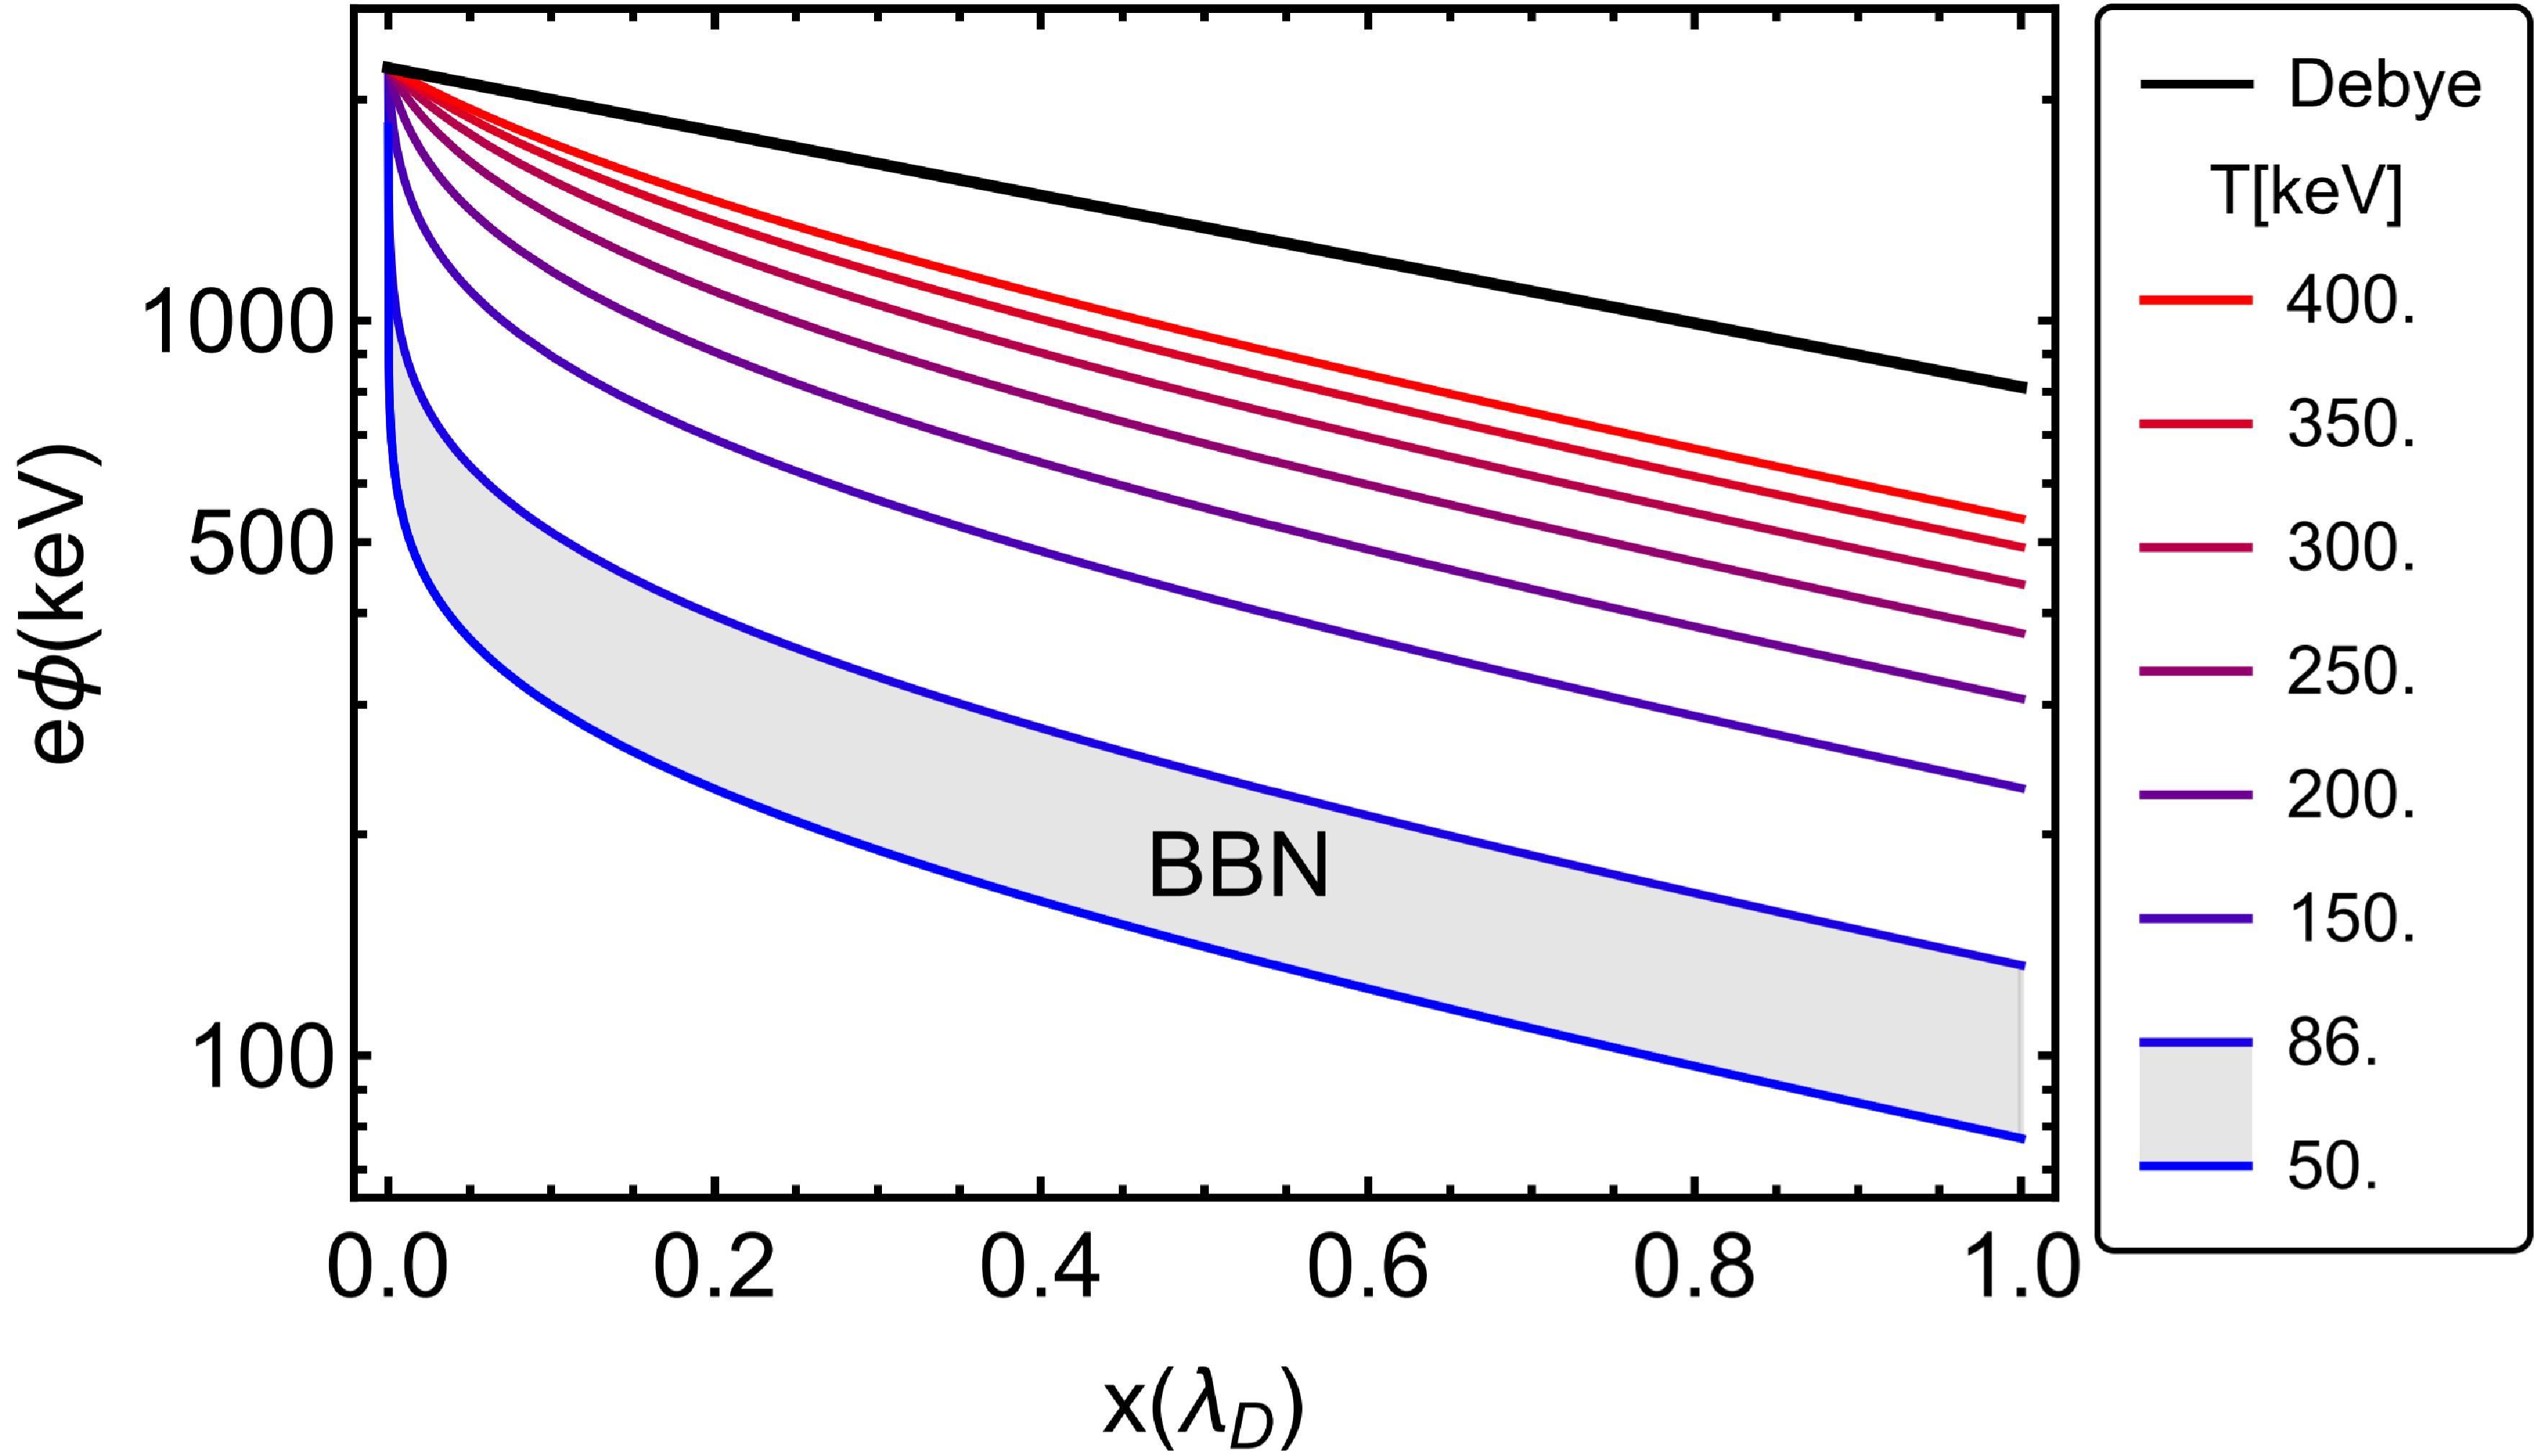
\includegraphics[width=.95\linewidth]{plots/chap03BBN/nonLinScreen.jpg}
%  \caption{Comparison of nonlinear screening to Debye linearized screening (solid top line) in the range $50\le T\le 400$\,keV; the BBN temperature range is shaded. In this toy model example $Z=2$ was used in \req{eq:phi0}.
%  } \label{fig:nonlinscreen}
% \end{figure}

% We contrast linear screening \req{eq:linscreen} and nonlinear screening \req{eq:nonlinscreen} in \reff{fig:nonlinscreen}. The boundary value of the potential $\phi_0$ is chosen to be the maximum value of the potential of a Gaussian charge distribution
% \begin{equation}\label{eq:phi0}
%  \phi_0 = \frac{Z e}{8 \pi^{3/2} \varepsilon_0 R}\,.
% \end{equation}
% Figure \ref{fig:nonlinscreen} shows that nonlinear screening and linear screening predict different decay rates for the potential $\phi$ at short distances but have the same long-range decay rate. Since the screening near the origin is larger in the nonlinear case, the long-distance potential $\phi$ does not approach the weak field limit but is offset. As \reff{fig:nonlinscreen} demonstrates this is especially true in the BBN temperature range. All solutions have an exponential slope $-m_D$ indicating linear or weak field behavior at large distances.

% The important prediction of the nonlinear screening in \reff{fig:nonlinscreen} is a rapid drop of the potential at short distances, thus a strong screening effect near the classical turning point of thermal reacting ions, where quantum tunneling for thermonuclear reactions will be important. This effect increases nonlinearly with $Z$, see \req{eq:nonlinscreen}. Note that the use of relativistic Fermi statistics may be required since the tunneling regime involves potentials that are comparable to and larger than the electron mass. We expect that nonlinear screening effects could lead to drastic changes in the Coulomb penetration factor for $Z>1$ and, in turn, light element abundances. 

% To describe nonlinear screening beyond the presented toy model, in the context of light element screening during BBN, we need to solve \req{eq:Poisson-Boltz} with a realistic spherical charge distribution. That way the difference in asymptotic behavior will be captured for the solution at large distances. It turns out that even the simple first look at the 3D-static asymptotic Debye-type solution requires formidable numerical effort, let alone merging the short-range strong field limit with damped-dynamic linear response theory as developed here. Therefore the strong field screening will be addressed separately, opening the path to the computation of screened-BBN reaction rates.

%%%%%%%%%%%%%%%%%%%%%%%%%%%%%%%%%%%%%%%%%%%%
\section{Dynamic screening in BBN: discussion and outlook}\label{sec:Discussion}

In this chapter, we reviewed \cite{Grayson:2023flr} which applies the non-relativistic longitudinal polarization function to study the dynamics of the electron-positron plasma in the early Universe. In particular, we discussed the damping rate, the electron-positron to baryon density ratio, and their potential implications for Big Bang Nucleosynthesis (BBN) through screening within linear response theory. We derived an approximate analytic formula for the potential of a moving heavy charge in a collisional plasma in \req{eq:pos_point_DDS} describing screening effects previously found only numerically \cite{Hwang:2021kno}. Our analytic formula can be readily used to estimate the effect of screening on thermonuclear reactions using \req{eq:DDSenhance}. The correction to thermonuclear reactions due to damped-dynamic screening is small due to the low velocity of nuclei and a large amount of collisional scattering. This is in line with the findings of \cite{Hwang:2021kno}, who conclude that even though the densities are large, they are not enough to modify the potential at short distances related to screening. The analytic expression we find for the nuclear reaction rate enhancement \req{eq:DDSenhance} in a collisional plasma could be useful in other fusion environments such as stellar fusion and laboratory fusion experiments, such as those discussed in ~\cite{Labaune:2013dla, Margarone:2022mdpi}.

Overall we were very surprised to find that the screening effects in BBN were so small even in the static case,  considering that the number densities present during BBN are $\sim 10^4$ times normal matter. If we compare this to screening effects on Earth, we can see that although plasmas occur at lower densities, they also occur in much colder environments. The strength of the screening effect is related to the Debye mass
\begin{equation}
m_D^2 \sim \frac{n_\text{eq} }{T}\,,
\end{equation}
which is on the order of a few keV during BBN. On earth, $n_\text{eq}$ is decreased by $\sim 10^4$, but T is decreased by $\sim 10^6$. Thus, we would expect to see similar, if not larger, screening effects on Earth. For instance, the Debye screening length in extracellular fluid in the body is 8 \AA ngstrom \cite{doi:10.1073/pnas.1914599117}, only a factor of $\sim 20$ times larger than the Debye length during BBN. We can have these large densities at low temperatures on earth due to gravity's agglomeration of matter in the universe.
\subsection{The short-range screening potential}
In \cite{Grayson:2023flr}, a proposal is made to study the short-range potential relevant to quantum tunneling in thermonuclear reactions. Since the Gamow energy at which nuclei are most likely to tunnel is above the thermal energy, the portion of the screening potential relevant for tunneling does not satisfy the "weak-field" limit where the electromagnetic energy is small compared to the thermal energy
\begin{equation}
    \frac{q \phi(x)}{T} \ll 1\,.
\end{equation}
When this condition is not satisfied one must consider the full equilibrium distribution when calculating the short-range potential \cite{Hakim:1967prd, DeGroot:1980dk}
\begin{equation}\label{eq:Boltz}
     f_B^\pm(x,p) = e^{-(p_0\pm e\phi(x))/T}\,.
\end{equation}
The $e\phi$ term in the exponential accounts for the change in energy of a charge in the plasma due to its presence in an external field. For this equilibrium distribution, a linear response is no longer possible since the equilibrium distribution depends on the external electromagnetic field. In equilibrium one can find the static screening potential for strong electromagnetic fields using the nonlinear Poisson-Boltzmann equation,
\begin{equation}\label{eq:Poisson-Boltz}
  -\nabla^2 e\phi_{(\text{eq})}(x)/T +m_D^2\sinh\left[e\phi_{(\text{eq})}(x)/T\right] =e\rho_\mathrm{ext}(x)/T\,.
 \end{equation}
This equation has a well-known solution for an infinite sheet which we used to argue the importance of strong screening in BBN. 
In a future publication, we will solve the Poisson-Boltzmann equation with strong screening to calculate the short-range screening potential in BBN. We note that the toy model in \cite{Grayson:2023flr} overestimates strong screening effects for two reasons: an infinite sheet has a constant electric field requiring more polarizing charge density to screen the field, and the Boltzmann distribution in \req{eq:Boltz} does not account for the stacking of electron-positron states when the density of electrons and positrons becomes very large near the nucleus. Both of these effects significantly reduce the effect of strong screening on reaction rates, but at the time of writing, it seems that strong screening will create a larger effect on nuclear reaction rates than damped-dynamic screening. Predicting enhanced screening may be relevant for the anomalous screening observed in the measurements of astrophysical S(E) factors \cite{Zhang_2020}.


\subsection{Dusty plasmas}
In \cite{Grayson:2023flr} were very interested in finding BBN plasma had similar properties to planetary and space dusty plasma theory~\cite{Montgomery:1970jpp, Stenflo:1973, Shukla:2002ppcf, Lampe:2000pop}. The large distance behavior of the damped-dynamic BBN screened potential in \req{eq:pos_point_DDS} matched that of slowly moving dust particles in plasma \cite{Stenflo:1973}. Dusty plasma theory studies many effects not currently included in BBN plasma studies, including dust charging, dust acoustic waves, dust instabilities, and structure formation (dust crystals)~\cite{Shukla:2002ppcf}. We expect that these results can be ported to the nuclear light element dust dynamics in the primordial $e^-e^+\gamma$ QED plasma. This interdisciplinary connection, which has not been recognized previously, could have substantial implications for our understanding of the evolution of matter in the early Universe.

\subsection{Structure formation in the early universe}
One may note that the portion of the screening potential in the direction of motion is slightly binding \reff{fig:dynamiclinear}.
Given recent observations from JWST \cite{ferreira2023jwst}, one could speculate that this polarization binding effect could lead to the early seeding of matter structure in the Universe. In dusty plasmas, this happens due to an attractive portion of the internuclear (charged dust) potential, which favors a specific average separation between charged dust particles. From the plasma parameters calculated in \cite{Grayson:2023flr} the depth of the binding potential is on the order of 10's of electron volts. While this is more energy than the usual molecular bond, the BBN temperature is likely too large for these binding energies to play a role in dynamics. Given the potential in \req{eq:pos_point_DDS}, calculating if a molecular bound state exists is the subject of future work.
\subsection{QGP in the early universe}
We hope to bridge Chapters 1 and 2 by studying QGP in the early universe. QGP filled the universe a few microseconds after the Big Bang \cite{rafelski2013connecting}. One could study the QCD potential of heavy quarks propagating through QGP in heavy ion collisions or the early universe. In dynamic screening of heavy quarks, it is possible that a long-range attractive potential also arises, leading to the formation of inhomogeneities in the early universe during the QGP epoch. In QCD, the transport equations are complicated by their non-abelian nature. Since gluons can couple to the external field of heavy quarks, they would contribute non-trivially to the transport equations. We expect we would also have to use strong-field kinetic theory due to the large QCD coupling $\alpha_s$. Kinetic theory in QGP is discussed in detail in \cite{MROWCZYNSKI20171}.

% \section*{Acknowledgements}
% This research did not receive any specific grant from funding agencies in the public, commercial, or not-for-profit sectors. However, we thank Tam\'as Bir\'o for his hospitality at the PP2023 Margaret Island Symposium where this work was presented. An allocation of computer time was used from the High Performance Computing (HPC) resources supported by the University of Arizona TRIF, UITS, and Research, Innovation, and Impact (RII) and maintained by the UArizona Research Technologies department.
% %%%%%%%%%%%%%%%%%%%%%%%%%%%%%%%%%%%%%%%%%%%%%%%%%%%%%%%%%%%%%%%%%%
% %===================================================================
% %===================================APPENDICES======================

% %===================================================================


% \section{External charge distribution}\label{sec:freechg}

% Here we define the free charge density used to describe light nuclei in BBN. We wish to model a nucleus moving at constant velocity $\boldsymbol{\beta}_N$. For simplicity, we model the charge distribution as a Gaussian in all directions
% \begin{equation}
% \rho_{\text{ext} }(t,\boldsymbol{x}) = \frac{Ze\gamma}{\pi^{3/2}R^3}e^{-\frac{1}{R^2}(\boldsymbol{x}-\boldsymbol{\beta}_N t )^2}\,,
% \end{equation}
% Since we work in the non-relativistic limit we assume that the Lorentz factor $\gamma\approx1$. The normalization is chosen in such a way that 
% \begin{equation}
% \int \rho_{\text{ext}}(t,\boldsymbol{x}) d^3\boldsymbol{x} = Ze\,
% \end{equation}
% is the total charge of the nucleus. The Gaussian radius parameter $R$ is related to the mean squared radius of the nucleus, $\langle r^2\rangle$ at rest, by
% \begin{equation}\label{eq:radius}
% \langle r^2 \rangle = \frac{1}{Ze}\int r^2 \rho_{\text{ext}}(\boldsymbol{x}) d^3\boldsymbol{x} = \frac{3}{2}R^2\,.
% \end{equation}
% Experimental measurements of the mean square radius can be found in Ref.~\cite{DeVries:1987atn}. The Fourier transformed charge distribution is
% \begin{equation}\label{eq:extchgfreq}
% \wt{\rho}_{\text{ext}}(\omega,\boldsymbol{k}) = 2\pi Ze\, e^{-\boldsymbol{k}^2 \frac{R^2}{4}} \delta(\omega - \boldsymbol{k}\cdot \boldsymbol{\beta}_N)\,,
% \end{equation} 
% where $\delta$ is the Dirac delta function in one dimension.

% \section{Static screening for a Gaussian charge distribution}\label{sec:static}
% Starting from \req{eq:potentk} we can take the limit $\beta_N\rightarrow0$ to find the static screening potential for a Gaussian charge distribution
% \begin{equation}
%  \phi_{\text{stat}}(t,\boldsymbol{x}) = Ze\int \frac{d^3\boldsymbol{k}}{(2\pi)^3} e^{ i\boldsymbol{k}\cdot \boldsymbol{x}} \frac{ e^{-\boldsymbol{k}^2\frac{R^2}{4}}}{\boldsymbol{k}^2+m_D^2}\,.
% \end{equation}
% First, we perform the angular integration to find
% \begin{equation}
%  \phi_{\text{stat}}(t,\boldsymbol{x}) = Ze\int_0^{\infty} \frac{k^2 d{k}}{(2\pi)^2} \frac{2\sin{({k}|\boldsymbol{x}|)}}{{k}|\boldsymbol{x}|} \frac{ e^{-{k}^2\frac{R^2}{4}}}{{k}^2+m_D^2}\,.
% \end{equation}
% This integral can be evaluated using a Schwinger parameterization
% \begin{equation}\label{eq:schwin}
%  \phi_{\text{stat}}(t,\boldsymbol{x}) = Ze\int_0^{\infty} ds \int_0^{\infty} \frac{k^2 d{k}}{(2\pi)^2} \frac{2\sin{({k}|\boldsymbol{x}|)}}{{k}|\boldsymbol{x}|} e^{-{k}^2\frac{R^2}{4}-s({{k}^2+m_D^2})}\,,
% \end{equation}
% where we first perform the integration over $k$. The $k$ integration is calculated by writing the $\sin$ in its exponential form and splitting it into two terms with opposite signs in the exponents. These two terms can be recombined into one Fourier transform from $-\infty$ to $+\infty$. Finally, the integration over $s$ results in the position space static screening potential
% \begin{multline}\label{eq:Stat_Gauss}
%  \phi_{\text{stat}}(t,\boldsymbol{x}) =\frac{Z e}{4 \pi \varepsilon_0}\frac{e^{m_D^2 R^2/4}}{r}\Bigg(\frac{ \text{Erf}\left(\frac{r}{R} - \frac{m_D R}{2}\right)}{2 }e^{-m_D r} \\+\frac{ \text{Erf}\left(\frac{r}{R} + \frac{m_D R}{2}\right)}{2 }e^{m_D r} - \sinh(m_D r)\Bigg)\,,
% \end{multline}
% where we have reintroduced the vacuum permittivity $\varepsilon_0$. Taking the limit of this expression for $R\rightarrow0$ yields the usual static screening result \cite{Debye:1923}
% \begin{equation}
%  \lim_{R\rightarrow 0} \phi_{\text{stat}}(t,\boldsymbol{x}) = \frac{Z e}{4 \pi \varepsilon_0}\frac{e^{-m_D r}}{r}\,.
% \end{equation}


%\newpage

% %%%%%%%%%%%%%%%%%%%%%%%%%%%%%%%%%%%%%%%%%%%%%%%%%%%%%%%%%%%%%%%%%%%%%%
% \begin{thebibliography}{99}

% \bibitem{Wang:2010px} 
% B.~Wang, C.~A.~Bertulani and A.~B.~Balantekin,
% \lq\lq Electron screening and its effects on Big-Bang nucleosynthesis,\rq\rq
% Phys.\ Rev.\ C {\bf 83}, 018801 (2011)
% doi:10.1103/PhysRevC.83.018801
% [arXiv:1010.1565 [astro-ph.CO]]

% \bibitem{Hwang:2021kno}
% E.~Hwang, D.~Jang, K.~Park, M.~Kusakabe, T.~Kajino, A.~B.~Balantekin, T.~Maruyama, C.~M.~Ryu and M.~K.~Cheoun,
% \lq\lq Dynamical screening effects on Big-Bang nucleosynthesis,\rq\rq
% JCAP \textbf{11} (2021), 017
% doi:10.1088/1475-7516/2021/11/017
% [arXiv:2102.09801 [nucl-th]]

% \bibitem{Rafelski:2023emw}
% J.~Rafelski, J.~Birrell, A.~Steinmetz and C.~T.~Yang,
% \lq\lq A short survey of matter-antimatter evolution in the primordial Universe,\rq\rq
% Universe \textbf{9}, 309 (2023)
% doi:10.3390/Universe9070309
%  [arXiv:2305.09055 [hep-th]]

% \bibitem{Salpeter:1954nc}
% E.~E.~Salpeter,
% \lq\lq Electron screening and thermonuclear reactions,\rq\rq
% Austral. J. Phys. \textbf{7} (1954), 373-388
% doi:10.1071/PH540373 

% \bibitem{Debye:1923}
% P. Debye and E. Hückel, 
% \lq\lq Zur Theorie der Elektrolyte,\rq\rq
% Physikalische Zeitschrift \textbf{24} 185–206 (1923).

% \bibitem{Salpeter:1969apj} 
% E.~E.~Salpeter and H.~M.~van Horn, 
% \lq\lq Nuclear Reaction Rates at High Densities,\rq\rq
% Astrophys. J., \textbf{155}, 183 (1969)
% doi:10.1086/149858

% \bibitem{Famiano:2016hhs}
% M.~A.~Famiano, A.~B.~Balantekin and T.~Kajino,
% \lq\lq Low-lying Resonances and Relativistic Screening in Big-Bang Nucleosynthesis,\rq\rq
% Phys. Rev. C \textbf{93} (2016) no.4, 045804
% doi:10.1103/PhysRevC.93.045804
% [arXiv:1603.03137 [astro-ph.CO]]

% \bibitem{Carraro:1988apj} 
% C. Carraro, A. Schafer and S. E. Koonin, 
% \lq\lq Dynamic Screening of Thermonuclear Reactions,\rq\rq 
% Astrophys. J., \textbf{331}, 565 (1988) 
% doi:10.1086/166582

% \bibitem{Gruzinov:1997as}
% A.~V.~Gruzinov,
% \lq\lq Dynamic screening and thermonuclear reaction rates,\rq\rq
% Astrophys. J. \textbf{496} (1998), 503
% doi:10.1086/305349
% [arXiv:astro-ph/9702064 [astro-ph]]

% \bibitem{Opher:1999jh}
% M.~Opher and R.~Opher,
% ``Dynamic screening in thermonuclear reactions,''
% Astrophys. J. \textbf{535} (2000), 473-474
% doi:10.1086/308808
% [arXiv:astro-ph/9908218 [astro-ph]].

% \bibitem{Yao:2016cjs}
% X.~Yao, T.~Mehen and B.~M\"uller,
% ``Dynamical screening of \ensuremath{\alpha}-\ensuremath{\alpha} resonant scattering and thermal nuclear scattering rate in a plasma,''
% Phys. Rev. D \textbf{95} (2017) no.11, 116002
% doi:10.1103/PhysRevD.95.116002
% [arXiv:1609.00383 [nucl-th]].

% \bibitem{Sasankan:2019oee}
% N.~Sasankan, A.~Kedia, M.~Kusakabe and G.~J.~Mathews,
% `Analysis of the Multi-component Relativistic Boltzmann Equation for Electron Scattering in Big Bang Nucleosynthesis,''
% Phys. Rev. D \textbf{101} (2020) no.12, 123532
% doi:10.1103/PhysRevD.101.123532
% [arXiv:1911.07334 [nucl-th]].

% \bibitem{Kedia:2020xdc}
% A.~Kedia, N.~Sasankan, G.~J.~Mathews and M.~Kusakabe,
% ``Simulations of Multi-Component Relativistic Thermalization,''
% Phys. Rev. E \textbf{103} (2021), 032101
% doi:10.1103/PhysRevE.103.032101
% [arXiv:2004.13186 [cond-mat.stat-mech]].


% \bibitem{Pitrou:2018cgg}
% C.~Pitrou, A.~Coc, J.~P.~Uzan and E.~Vangioni,
% \lq\lq Precision big bang nucleosynthesis with improved Helium-4 predictions,\rq\rq
% Phys. Rept. \textbf{754}, 1-66 (2018)
% doi:10.1016/j.physrep.2018.04.005
% [arXiv:1801.08023 [astro-ph.CO]]
 
% \bibitem{Pitrou:2021vqr}
% C.~Pitrou, A.~Coc, J.~P.~Uzan and E.~Vangioni,
% \lq\lq Resolving conclusions about the early Universe requires accurate nuclear measurements,\lq\lq
% Nature Rev. Phys. \textbf{3},  231 (2021)
% doi:10.1038/s42254-021-00294-6
% [arXiv:2104.11148 [astro-ph.CO]] 

% \bibitem{Bertulani:2022qly}
% C.~A.~Bertulani, F.~W.~Hall and B.~I.~Santoyo,
% \lq\lq Big Bang nucleosynthesis as a probe of new physics,\rq\rq
% EPJ Web Conf. \textbf{275}, 01003 (2023)
% doi:10.1051/epjconf/202327501003
% [arXiv:2210.04071 [nucl-th]]

% \bibitem{Meissner:2023voo}
% U.~G.~Mei\ss{}ner, B.~C.~Metsch and H.~Meyer,
% \lq\lq The electromagnetic fine-structure constant in primordial nucleosynthesis revisited,\rq\rq
% [arXiv:2305.15849 [hep-th]]

% \bibitem{Haro:2023JWST}
% P.~A.~Haro et al,
% \lq\lq Spectroscopic verification of very luminous galaxy candidates in the early universe,\rq\rq
% [arXiv:2303.08918 [astro-ph.GA]]

% \bibitem{Sabti:2023xwo}
% N.~Sabti, J.~B.~Mu\~noz and M.~Kamionkowski,
% \lq\lq Insights from HST into Ultra-Massive Galaxies and Early-Universe Cosmology,\rq\rq
% [arXiv:2305.07049 [astro-ph.CO]].

% \bibitem{Ilie:2023DM}
% Cosmin Ilie, Jillian Paulin, and Katherine Freese,
% ``Supermassive Dark Star candidates seen by JWST,''
% PNAS \textbf{120}, e2305762120 (2023)
% doi:10.1073/pnas.2305762120
 

%  \bibitem{Bhatnagar:1954zz}
% P.~L.~Bhatnagar, E.~P.~Gross and M.~Krook,
% \lq\lq A Model for Collision Processes in Gases. 1. Small Amplitude Processes in Charged and Neutral One-Component Systems,\rq\rq
% Phys. Rev. \textbf{94}, 511 (1954)
% doi:10.1103/PhysRev.94.511 

% \bibitem{Formanek:2021blc}
% M.~Formanek, C.~Grayson, J.~Rafelski and B.~M\"uller,
% \lq\lq Current-conserving relativistic linear response for collisional plasmas,\rq\rq
% Annals Phys. \textbf{434} (2021), 168605
% doi:10.1016/j.aop.2021.168605
% [arXiv:2105.07897 [physics.plasm-ph]]


% \bibitem{Montgomery:1970jpp}
% D.~Montgomery, G.~Joyce, and R.~Sugihara,
% \lq\lq Inverse third power law for the shielding of test particles,\rq\rq
% J. Plasma Phys. {\bf 4}, 1-13 (1970)

% \bibitem{Stenflo:1973}
% L.~Stenflo, M.~Y.~Yu, and P.~K.~Shukla
% \lq\lq Shielding of a slow test charge in a collisional plasma\rq\rq
% Phys. Fluids \textbf{16}, 450 (1973)
% doi:10.1063/1.1694361

% \bibitem{Shukla:2002ppcf}
% P.~K.~Shukla and A.~A.~Mamun
% \lq\lq Introduction to Dusty Plasma Physics\rq\rq
% Plasma Phys. Control. Fusion 44 395 (2002)
% doi:10.1088/0741-3335/44/3/701

% \bibitem{Lampe:2000pop}
% Martin Lampe, Glenn Joyce, Gurudas Ganguli and Valeriy Gavrishchaka
% \lq\lq Interactions between dust grains in a dusty plasma\rq\rq
% Physics of Plasmas \textbf{7}, 3851 (2000) 
% doi:10.1063/1.1288910

% \bibitem{Grayson:2022asf}
% C.~Grayson, M.~Formanek, J.~Rafelski and B.~Mueller,
% \lq\lq Dynamic magnetic response of the quark-gluon plasma to electromagnetic fields,\rq\rq
% Phys. Rev. D \textbf{106} (2022) no.1, 014011
% doi:10.1103/PhysRevD.106.014011
% [arXiv:2204.14186 [hep-ph]]
 
% \bibitem{Birrell:2012gg} 
% J.~Birrell, C.~T.~Yang, P.~Chen and J.~Rafelski,
% \lq\lq Relic neutrinos: Physically consistent treatment of effective number of neutrinos and neutrino mass,\rq\rq
% Phys.\ Rev.\ D {\bf 89}, 023008 (2014)
% doi:10.1103/PhysRevD.89.023008

% \bibitem{ParticleDataGroup:2022pth}
% R.~L.~Workman \textit{et al.} [Particle Data Group],
% \lq\lq Review of Particle Physics,\rq\rq
% PTEP \textbf{2022}, 083C01 (2022)
% doi:10.1093/ptep/ptac097

% \bibitem{Letessier:2002gp}
% J.~Letessier and J.~Rafelski,
% \textit{Hadrons and quark-gluon plasma,\/} 
% %Camb.\ Monogr.\ Part.\ Phys.\ Nucl.\ Phys.\ Cosmol.\ \textbf{18}, 1-418 
% Cambridge University Press (2002, 2022)
% doi:10.1017/9781009290753 (Open Access)

% \bibitem{Kuznetsova:2009bq}
% I.~Kuznetsova, D.~Habs and J.~Rafelski,
% \lq\lq Thermal reaction processes in a relativistic QED plasma drop,\rq\rq
% Phys. Rev. D \textbf{81}, 053007 (2010)
% doi:10.1103/PhysRevD.81.053007

% \bibitem{Kuznetsova:2011wt}
% I.~Kuznetsova and J.~Rafelski,
% \lq\lq Electron-Positron Plasma Drop Formed by Ultra-Intense Laser Pulses,\rq\rq
% Phys. Rev. D \textbf{85}, 085014 (2012)
% doi:10.1103/PhysRevD.85.085014

% \bibitem{Kislinger:1975uy}
% M.~B.~Kislinger and P.~D.~Morley,
% \lq\lq Collective Phenomena in Gauge Theories. 1. The Plasmon Effect for Yang-Mills Fields,\rq\rq
% Phys. Rev. D \textbf{13}, 2765 (1976)
% doi:10.1103/PhysRevD.13.2765

% \bibitem{Starke:2014tfa}
% R.~Starke and G.~A.~H.~Schober,
% \lq\lq Relativistic covariance of Ohm's law,\rq\rq
% Int. J. Mod. Phys. D \textbf{25}, 1640010 (2016)
% doi:10.1142/S0218271816400101
% [arXiv:1409.3723 [math-ph]]

% \bibitem{melrose2008quantum}
% D.~Melrose,
% {\it Quantum Plasmadynamics: Unmagnetized Plasmas},
% Lect. Notes Phys. \textbf{735} 
% (Springer, New York, 2008)
% doi:10.1007/978-0-387-73903-8

%  %\cite{Steinmetz:2023abc}
% \bibitem{Steinmetz:2023abc}
% A.~Steinmetz, C.~T.~Yang, and J.~Rafelski,
% \lq\lq Matter-antimatter origin of cosmic magnetism,\rq\rq
% [arXiv:2308.14818 [hep-ph]]

% \bibitem{Shukla1996}
% P.~K.~Shukla and N.~N.~Rao
% \lq\lq Coulomb crystallization in colloidal plasmas with streaming ions and dust grains\rq\rq
% Physics of Plasmas \textbf{3}, 1770 (1996)
% doi: 10.1063/1.871695

% \bibitem{Hakim:1967prd}
% R.~Hakim
% \rq\rq Relativistic Perfect Gas in an External Force Field,\rq\rq
% Phys. Rev. \textbf{162}, 128 (1967)
% doi:10.1103/PhysRev.162.128


% \bibitem{DeGroot:1980dk}
% S.~R.~De Groot, W.~A.~Van Leeuwen and C.~G.~Van Weert,
% \textit{Relativistic Kinetic Theory. Principles and Applications,} 
% North-Holland Publishing Company (1980)


% \bibitem{Gouy:1910}
% G.~Gouy
% \lq\lq Sur la constitution de la charge \'electrique \`a la surface d’un \'electrolyte,\rq\rq
% J. Phys. Theor. Appl., \textbf{9} , 457 (1910)
% doi:10.1051/jphystap:019100090045700 

% \bibitem{Thomas:1994prl}
% H.~Thomas, G.~E.~Morfill, V.~Demmel, J.~Goree, B.~Feuerbacher and D.~M\"ohlmann,
% \lq\lq Plasma Crystal: Coulomb Crystallization in a Dusty Plasma,\rq\rq
% Phys. Rev. Lett. \textbf{73}, 652 (1994) 
% doi:10.1103/PhysRevLett.73.652

% \bibitem{Gupta:2023mn}
% R.~Gupta,
% ``JWST early Universe observations and $\Lambda$CDM cosmology''
% %Monthly Notices of the Royal Astronomical Society, 
% MNRAS stad2032, (2023)
% doi:10.1093/mnras/stad2032

% \bibitem{Labaune:2013dla}
% C.~Labaune, C.~Baccou, S.~Depierreux, C.~Goyon, G.~Loisel, V.~Yahia and J.~Rafelski,
% \lq\lq Fusion reactions initiated by laser-accelerated particle beams in a laser-produced plasma,\rq\rq
% Nature Commun. \textbf{4}, 2506 (2013)
% doi:10.1038/ncomms3506
% [arXiv:1310.2002 [physics.plasm-ph]]


%  \bibitem{Margarone:2022mdpi}
%  Daniele Margarone, Julien Bonvalet, Lorenzo Giuffrida, Alessio Morace, Vasiliki Kantarelou, Marco Tosca, Didier Raffestin, Philippe Nicolai, Antonino Picciotto, Yuki Abe, Yasunobu Arikawa, Shinsuke Fujioka, Yuji Fukuda, Yasuhiro Kuramitsu, Hideaki Habara and Dimitri Batani,
%  \lq\lq In-Target Proton–Boron Nuclear Fusion Using a PW-Class Laser,\rq\rq
%  MDPI Applied Sciences , \textbf{12}(3), [e1444].
%  doi:10.3390/app12031444 
 
% \bibitem{Buyukcizmeci:2023azb}
% N.~Buyukcizmeci, T.~Reichert, A.~S.~Botvina and M.~Bleicher,
% \lq\lq Nucleosynthesis of light nuclei and hypernuclei in central Au+Au collisions at $\sqrt{s_{NN}}$=3 GeV,\rq\rq
% [arXiv:2306.17145 [nucl-th]]


% \bibitem{Zhao:2020jqu}
% J.~Zhao, K.~Zhou, S.~Chen and P.~Zhuang,
% \lq\lq Heavy flavors under extreme conditions in high energy nuclear collisions,\rq\rq
% Prog. Part. Nucl. Phys. \textbf{114}, 103801 (2020)
% doi:10.1016/j.ppnp.2020.103801
% [arXiv:2005.08277 [nucl-th]]
 
% \bibitem{DeVries:1987atn}
% H.~De Vries, C.~W.~De Jager and C.~De Vries,
% \lq\lq Nuclear charge and magnetization density distribution parameters from elastic electron scattering,\rq\rq
% Atom. Data Nucl. Data Tabl. \textbf{36}, 495 (1987)
% doi:10.1016/0092-640X(87)90013-1 


% %\bibitem{Yao:2016cjs}
% %X.~Yao, T.~Mehen and B.~M\"uller,
% %``Dynamical screening of \ensuremath{\alpha}-\ensuremath{\alpha} resonant scattering and thermal nuclear scattering rate in a plasma,''
% %Phys. Rev. D \textbf{95}, no.11, 116002 (2017)
% %doi:10.1103/PhysRevD.95.116002
% %[arXiv:1609.00383 [nucl-th]].

% \end{thebibliography}
% %%%%%%%%%%%%%%%%%%%%%%%%%%%%%%%%%%%%%%%%%%%%%%%%%%%%%%%%%%%%%%%%%%%
